\documentclass[12pt,a4paper]{article}

\usepackage[utf8]{inputenc}
\usepackage[T1]{fontenc}
\usepackage[spanish]{babel}
\usepackage{amsmath,amssymb}
\usepackage{graphicx}
\usepackage{array}
\usepackage[margin=2.5cm]{geometry}


%\lhead{Pr\'actica de Laboratorio Nuclear}

\title{\vspace{-1.5cm}\textbf{Pr\'actica de Coincidencias Gamma}\\
       \large An\'alisis de coincidencias $\gamma$-$\gamma$ con detectores NaI\\[0.3cm]
       \normalsize\textit{Informe de resultados experimentales}}

\author{Laboratorio de F\'isica Nuclear}
\date{\today}

\begin{document}
\maketitle
\thispagestyle{empty}

% ==============================================================================
\section*{Resumen}
% ==============================================================================

Se analizaron espectros de coincidencias $\gamma$-$\gamma$ de las fuentes de $^{22}$Na y $^{60}$Co,
adquiridos con un sistema digital XIA Pixie4 acoplado a detectores NaI.
Se identificaron y ajustaron picos de coincidencias reales (511\,keV y 1274\,keV para $^{22}$Na;
1173\,keV y 1332\,keV para $^{60}$Co) y se cuantific\'o la contribuci\'on de coincidencias accidentales.
El ajuste se realiz\'o mediante el m\'etodo de transformaci\'on logar\'tmica implementado en
Fortran (\texttt{src/gaussian\_background.f} y \texttt{src/subrutina.f}), que estima un fondo
lineal, lo sustrae, y ajusta una par\'abola a $\ln Y$ vs.\ $x$ para extraer los par\'ametros
gaussianos.
Se determin\'o la relaci\'on $R = N_{\text{acc}}(157^\circ)/N_{511+511}(180^\circ) = 0.071$,
y se analiz\'o el fondo ambiental mediante mediciones con $^{60}$Co y fondo puro (F+F).
Se discute la interpretaci\'on f\'isica de coincidencias reales y accidentales
en funci\'on de la geometr\'a de detecci\'on.

\newpage
\setcounter{section}{1}

% ==============================================================================
\section{Introducci\'on}
% ==============================================================================

La espectroscop\'a de coincidencias $\gamma$-$\gamma$ permite estudiar desintegraciones nucleares
en cascada, identificando eventos en los que dos o m\'as fotones son emitidos desde el mismo
n\'ucleo en un intervalo de tiempo corto (ventana de coincidencia, t\'picamente del orden de
decenas de nanosegundos a microsegundos).

El $^{22}$Na es un emisor $\beta^+$ que decae a $^{22}$Ne$^*$:
\begin{equation}
{}^{22}\text{Na} \xrightarrow{\beta^+} {}^{22}\text{Ne}^* \xrightarrow{\gamma} {}^{22}\text{Ne}
\end{equation}
El positr\'on se aniquila produciendo dos fotones de 511\,keV emitidos a 180$^\circ$ entre s\'i
(para conservar el momento lineal). El $^{22}$Ne$^*$ se desexcita emitiendo un fot\'on de
1274\,keV. Por tanto, en cada desintegraci\'on se producen tres fotones: dos de 511\,keV y
uno de 1274\,keV.

El $^{60}$Co decae por emisi\'on $\beta^-$ a $^{60}$Ni$^*$, emitiendo dos fotones en cascada
de 1173\,keV y 1332\,keV, \'utiles para calibraci\'on y estudio de correlaci\'on angular.

Los objetivos de este an\'alisis son:
\begin{enumerate}
  \item Identificar y ajustar los picos de coincidencia en espectros de $^{22}$Na a 157$^\circ$ y 180$^\circ$.
  \item Distinguir coincidencias reales de accidentales mediante el cociente $R$.
  \item Cuantificar la contribuci\'on del fondo ambiental usando $^{60}$Co y F+F.
  \item Interpretar f\'isicamente los resultados en funci\'on de la cinem\'atica de la desintegraci\'on y la geometr\'a del experimento.
\end{enumerate}

% ==============================================================================
\section{Configuraci\'on experimental}
% ==============================================================================

Los datos fueron adquiridos con un sistema digital XIA Pixie4 (4 canales) conectado a detectores
NaI. El sistema registra un espectro de amplitud (MCAch0) que histograma la energ\'a depositada
en el detector 0 \'unicamente cuando se produce un evento de coincidencia con el detector 1
dentro de la ventana de coincidencia configurada en el m\'odulo Pixie4.

Las mediciones realizadas fueron:
\begin{itemize}
  \item $^{22}$Na a 157$^\circ$: 651.2\,s, tasa~25.9\,cps.
  \item $^{22}$Na a 180$^\circ$: 313.9\,s, tasa~266.2\,cps.
  \item $^{60}$Co+F (fondo con fuente): 22607\,s, tasa~0.707\,cps.
  \item F+F (fondo sin fuente): 148117\,s, tasa~0.515\,cps.
\end{itemize}

\begin{table}[htbp]
\centering
\caption{Resumen de los espectros adquiridos.}
\label{tab:resumen}
\begin{tabular}{lcccc}
\hline \hline
Espectro & $t_{\text{real}}$ (s) & $t_{\text{vivo}}$ (s) & Tasa evento (cps) & \'Angulo \\
\hline
$^{22}$Na-157-coin & 651.2 & 651.2 & 25.91 & 157$^\circ$ \\
$^{22}$Na-180-coin & 313.9 & 313.9 & 266.17 & 180$^\circ$ \\
$^{60}$Co+F-coin    & 22607.4 & 22607.4 & 0.707 & --- \\
F+F-coin           & 148117.0 & 148117.0 & 0.515 & --- \\
\hline
\end{tabular}
\end{table}

% ==============================================================================
\section{Metodolog\'a de an\'alisis}
% ==============================================================================

\subsection{Ajuste de picos mediante transformaci\'on logar\'tmica}

El ajuste de picos se realiz\'o utilizando los c\'odigos Fortran en \texttt{src/},
que implementan un m\'etodo cl\'asico de tres etapas:

\textbf{Etapa 1 -- Fondo lineal:} Se identifican los puntos fuera de la regi\'on del pico
($x \le x_{\text{inicio}}$ o $x \ge x_{\text{fin}}$) y se ajusta un fondo lineal:
\begin{equation}
B(x) = a_{\text{bg}} + b_{\text{bg}}\,x
\end{equation}
por m\'inimos cuadrados lineales (subrutina \texttt{LFIT} de \texttt{subrutina.f}).

\textbf{Etapa 2 -- Transformaci\'on logar\'tmica:} Se resta el fondo y se toma logaritmo
natural de los datos netos:
\begin{equation}
Y_{\text{net}}(x) = Y(x) - B(x), \qquad Z(x) = \ln Y_{\text{net}}(x)
\end{equation}

\textbf{Etapa 3 -- Ajuste parab\'olico:} Se ajusta una par\'abola a $Z(x)$:
\begin{equation}
Z(x) = a + b\,x + c\,x^2
\end{equation}
usando \texttt{LFIT} con funciones base $\{1, x, x^2\}$.

Los par\'ametros gaussianos se extraen de los coeficientes:
\begin{align}
\sigma &= \sqrt{-\frac{1}{2c}} \\
x_0 &= b\,\sigma^2 \\
A &= \exp\!\left(a + \frac{x_0^2}{2\sigma^2}\right)
\end{align}
y el \'area neta del pico:
\begin{equation}
\text{\'Area} = A\,\sigma\sqrt{2\pi}
\end{equation}

Este m\'etodo (transformaci\'on logar\'tmica m\'as ajuste cuadr\'atico) es equivalente
a un ajuste gaussiano directo cuando el fondo se conoce con precisi\'on, y fue el
enfoque est\'andar en an\'alisis nucleares antes de la disponibilidad generalizada de
algoritmos de m\'inimos cuadrados no lineales.

\subsection{Coincidencias reales vs.\ accidentales}

En el espectro a 157$^\circ$, la coincidencia real es 511+1274, que produce igual n\'umero
de cuentas en ambos picos (es aleatorio qu\'e detector ve cada fot\'on). Por tanto:
\begin{itemize}
  \item $N_{511}(157^\circ)$: \'area neta del pico de 511\,keV a 157$^\circ$.
  \item $N_{1274}(157^\circ)$: \'area neta del pico de 1274\,keV a 157$^\circ$.
  \item $N_{\text{acc}}$: exceso de 511 sobre 1274 (coincidencias accidentales 511+511
        de dos desintegraciones distintas).
\end{itemize}
\begin{equation}
N_{\text{acc}}(157^\circ) = N_{511}(157^\circ) - N_{1274}(157^\circ)
\end{equation}

La relaci\'on de coincidencias accidentales se define como:
\begin{equation}
R = \frac{N_{\text{acc}}(157^\circ)}{N_{511+511}(180^\circ)}
\end{equation}

\subsection{An\'alisis de fondo}

Se utilizaron dos mediciones para caracterizar el fondo:
\begin{itemize}
  \item $^{60}$Co+F: incluye coincidencias reales de la cascada $^{60}$Co m\'as fondo.
  \item F+F: solo fondo ambiental (coincidencias accidentales).
\end{itemize}
La contribuci\'on del fondo se estima como:
\begin{equation}
\text{Fondo} = \frac{\text{tasa(F+F)}}{\text{tasa($^{60}$Co+F)}} \times 100\%
\end{equation}

% ==============================================================================
\section{Resultados}
% ==============================================================================

\subsection{Espectro completo de $^{22}$Na a 157$^\circ$}

\begin{figure}[htbp]
\centering
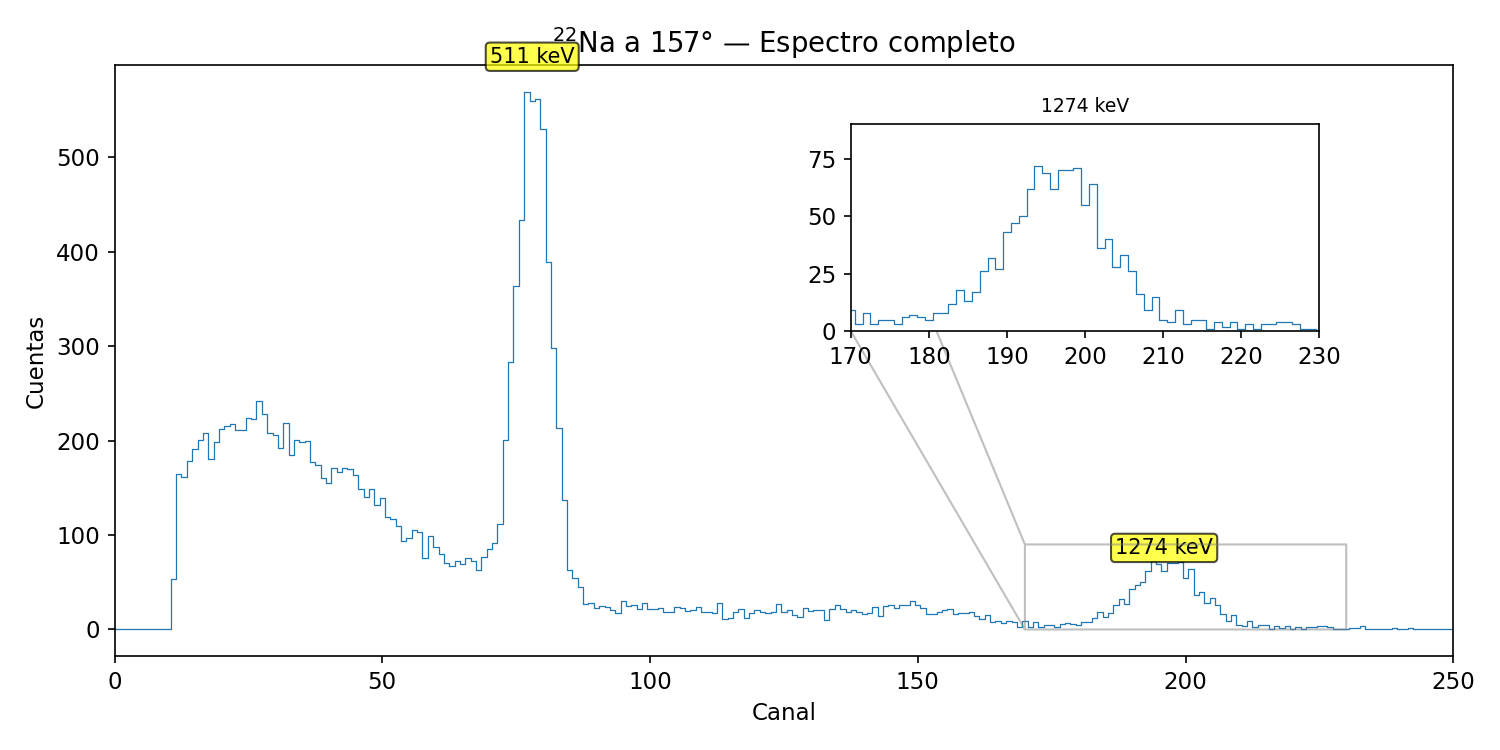
\includegraphics[width=\textwidth]{../graficos/ch0/22Na_157_completo.png}
\caption{Espectro completo de coincidencias de $^{22}$Na a 157$^\circ$. Se observan los picos de 511\,keV (canal~78) y 1274\,keV (canal~196). El recuadro muestra el detalle de la regi\'on de 1274\,keV.}
\label{fig:157_completo}
\end{figure}

El espectro a 157$^\circ$ (Fig.~\ref{fig:157_completo}) muestra dos picos claramente diferenciados.
A este \'angulo los detectores no pueden captar ambos fotones de aniquilaci\'on (que se emiten a 180$^\circ$),
por lo que la coincidencia se produce entre un fot\'on de 511\,keV y el de 1274\,keV.

\subsubsection{Pico de 511\,keV (canal~78)}

\begin{figure}[htbp]
\centering
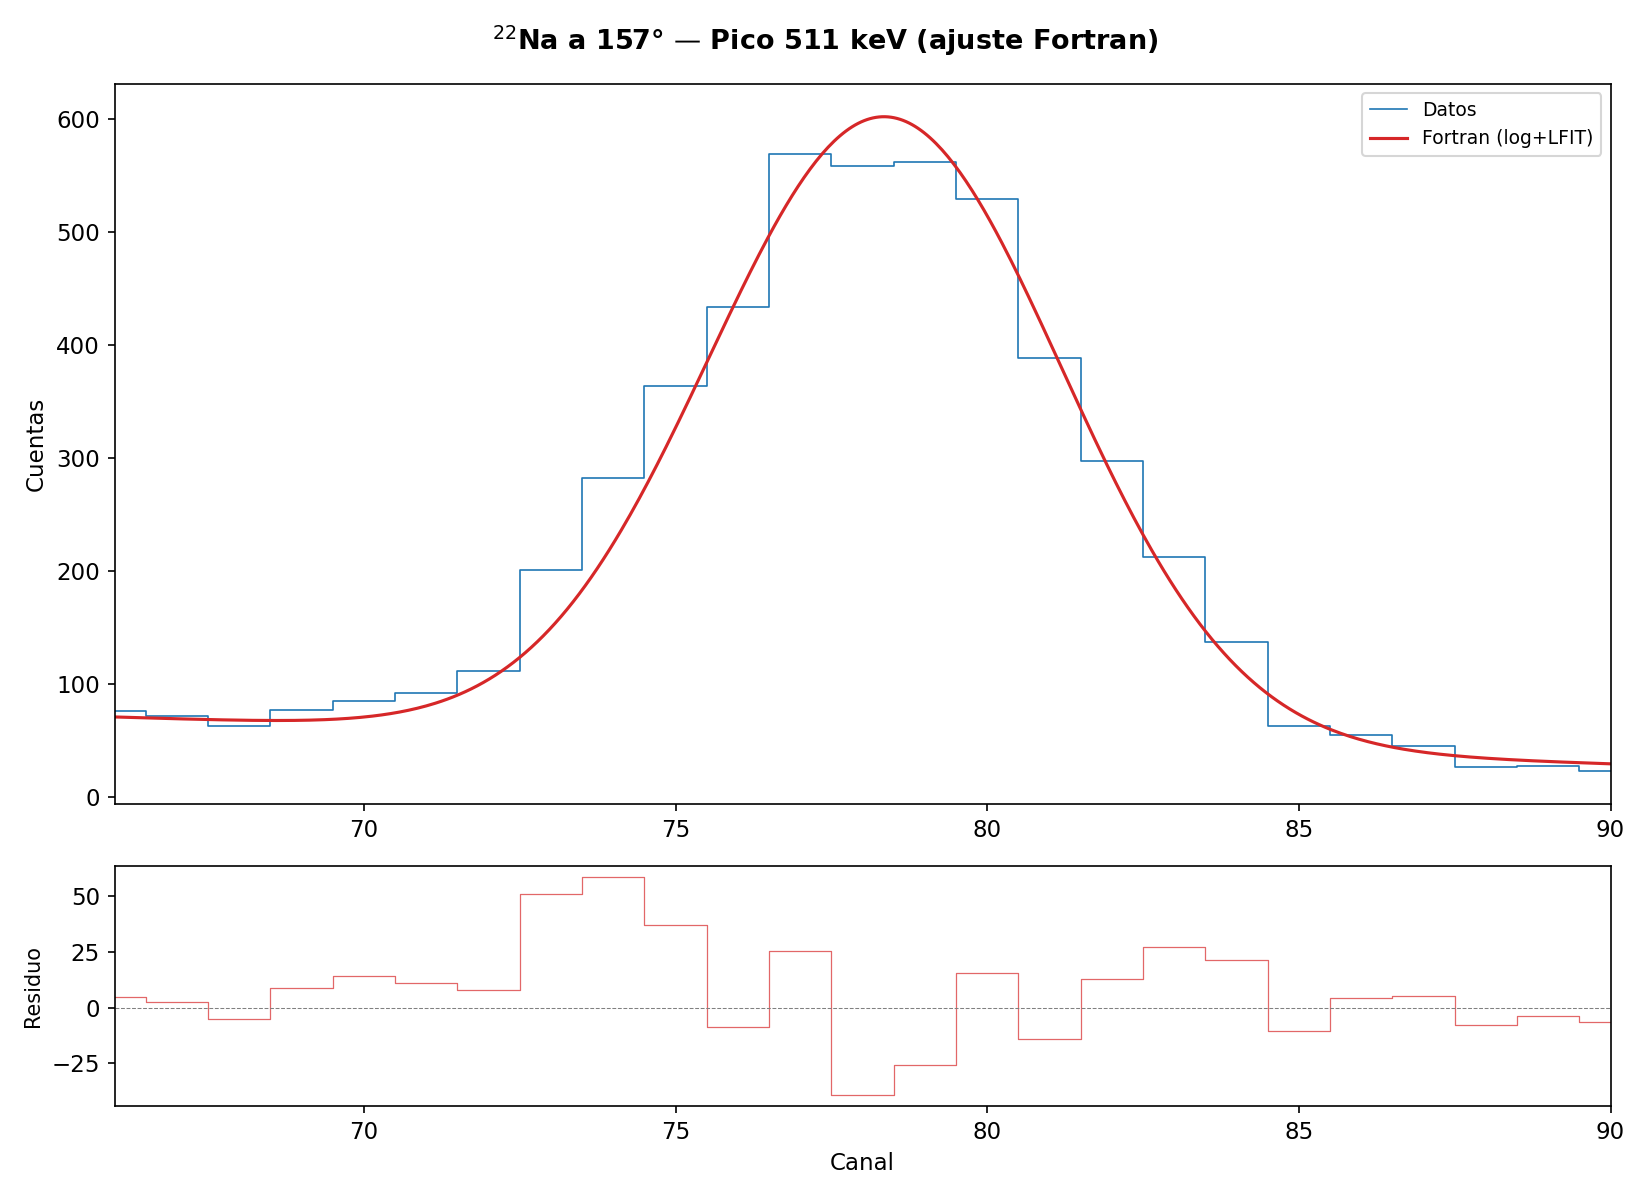
\includegraphics[width=0.85\textwidth]{../graficos/ch0/22Na_157_pico_511_1274.png}
\caption{Ajuste gaussiano del pico de 511\,keV en $^{22}$Na a 157$^\circ$. Se muestra el ajuste Fortran (l\'inea roja continua) y el ajuste Python/scipy (l\'inea verde discontinua) para comparaci\'on.}
\label{fig:511_157}
\end{figure}

\begin{table}[htbp]
\centering
\caption{Par\'ametros del ajuste del pico de 511\,keV a 157$^\circ$ (m\'etodo Fortran: fondo lineal + transformaci\'on logar\'tmica).}
\label{tab:511_157}
\begin{tabular}{lc}
\hline \hline
Par\'ametro & Valor \\
\hline
Centro $x_0$ (canal) & 78.37 \\
Desviaci\'on $\sigma$ (canal) & 2.83 \\
FWHM (canal) & 6.66 \\
Amplitud $A$ & 552.8 \\
\'Area neta & 3916 \\
\hline
\end{tabular}
\end{table}

\subsubsection{Pico de 1274\,keV (canal~196)}

\begin{figure}[htbp]
\centering
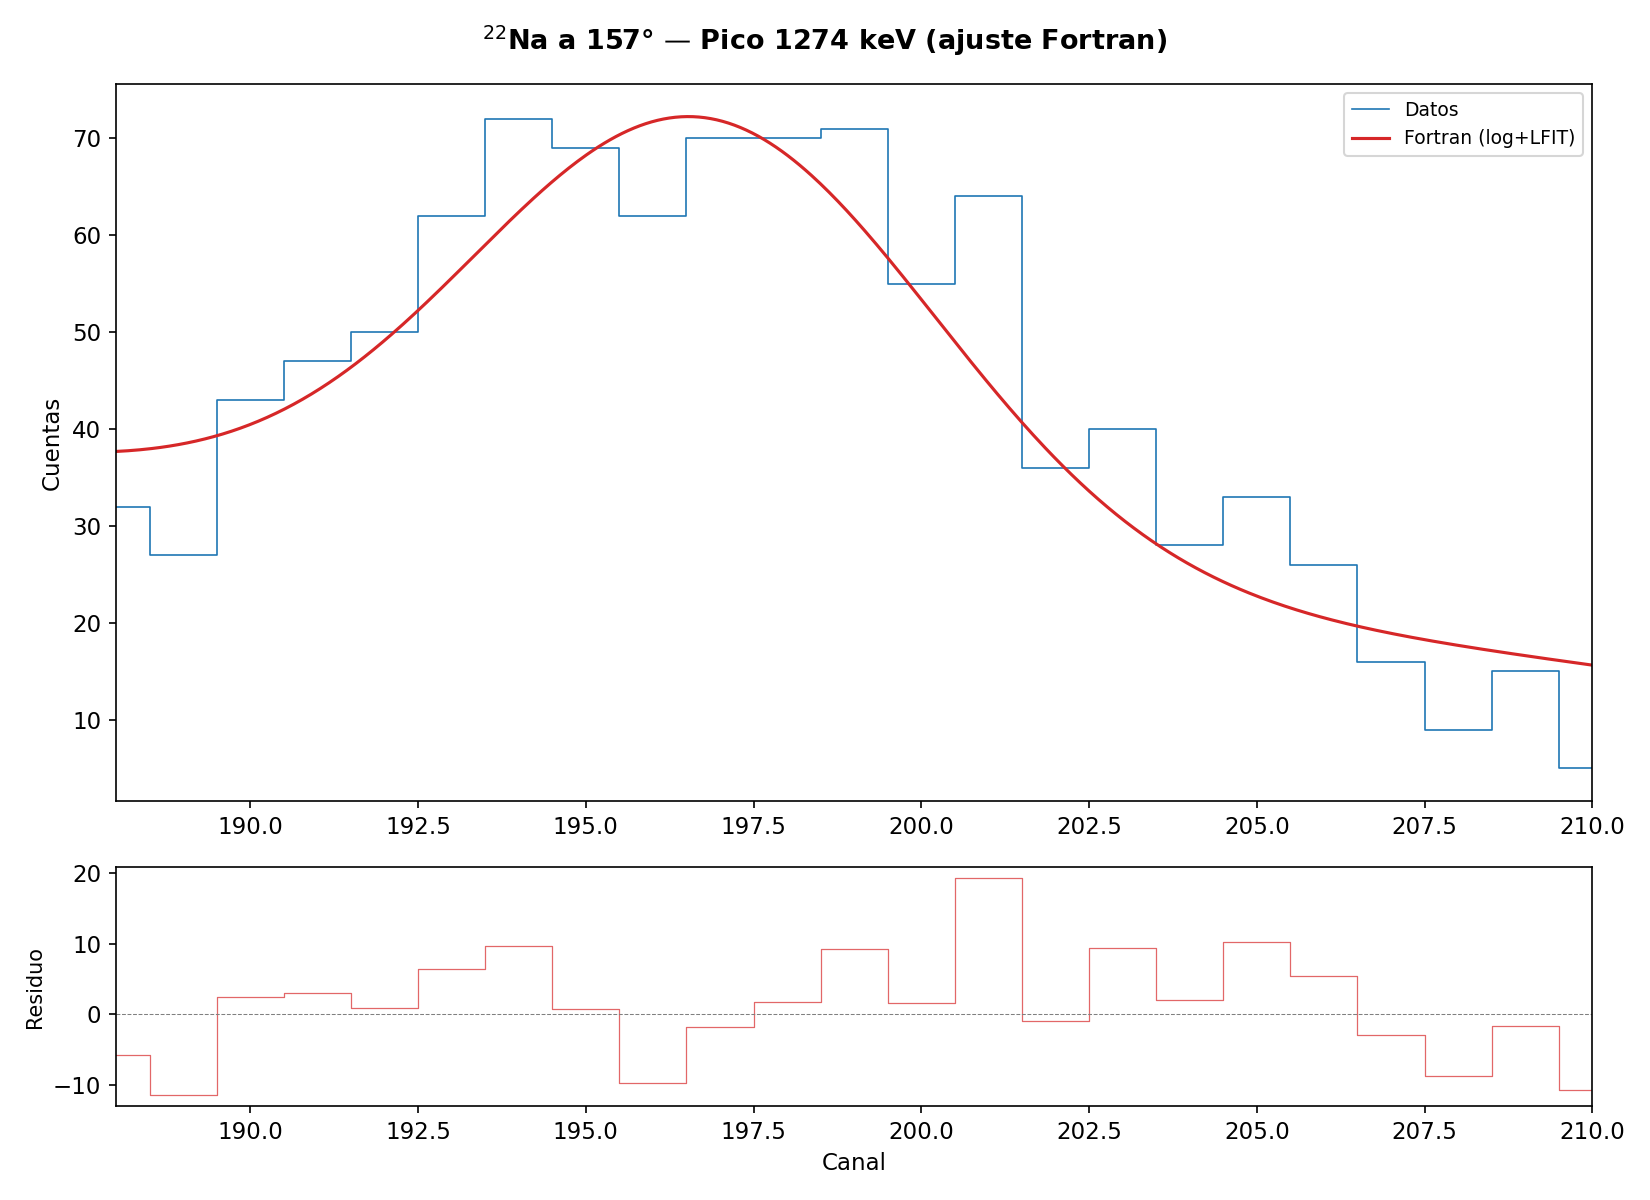
\includegraphics[width=0.85\textwidth]{../graficos/ch0/22Na_157_pico_1274.png}
\caption{Ajuste gaussiano del pico de 1274\,keV en $^{22}$Na a 157$^\circ$.}
\label{fig:1274_157}
\end{figure}

\begin{table}[htbp]
\centering
\caption{Par\'ametros del ajuste del pico de 1274\,keV a 157$^\circ$ (m\'etodo Fortran).}
\label{tab:1274_157}
\begin{tabular}{lc}
\hline \hline
Par\'ametro & Valor \\
\hline
Centro $x_0$ (canal) & 196.77 \\
Desviaci\'on $\sigma$ (canal) & 3.44 \\
FWHM (canal) & 8.10 \\
Amplitud $A$ & 44.2 \\
\'Area neta & 381 \\
\hline
\end{tabular}
\end{table}

\newpage
\subsection{Coincidencias a 157$^\circ$: reales vs.\ accidentales}

\begin{table}[htbp]
\centering
\caption{Resumen de cuentas en el espectro de $^{22}$Na a 157$^\circ$.}
\label{tab:cuentas_157}
\begin{tabular}{lc}
\hline \hline
Cantidad & Valor \\
\hline
$N_{\text{total}}(157^\circ)$ & 16873 \\
\'Area pico 511\,keV & 3916 \\
\'Area pico 1274\,keV & 381 \\
$N_{\text{acc}} = N_{511} - N_{1274}$ & 3535 \\
\hline
\end{tabular}
\end{table}

Las coincidencias accidentales ($N_{\text{acc}} = 3535$) corresponden al exceso de
cuentas en el pico de 511\,keV sobre el de 1274\,keV. Incluyen principalmente:
\begin{itemize}
  \item Coincidencias accidentales 511+511 de dos desintegraciones distintas.
  \item Eventos Compton de un fot\'on de 1274\,keV que se dispersa y es detectado
        simult\'aneamente con otro evento en el otro detector.
  \item Fondo ambiental.
\end{itemize}

\subsection{Espectro de $^{22}$Na a 180$^\circ$}

\begin{figure}[htbp]
\centering
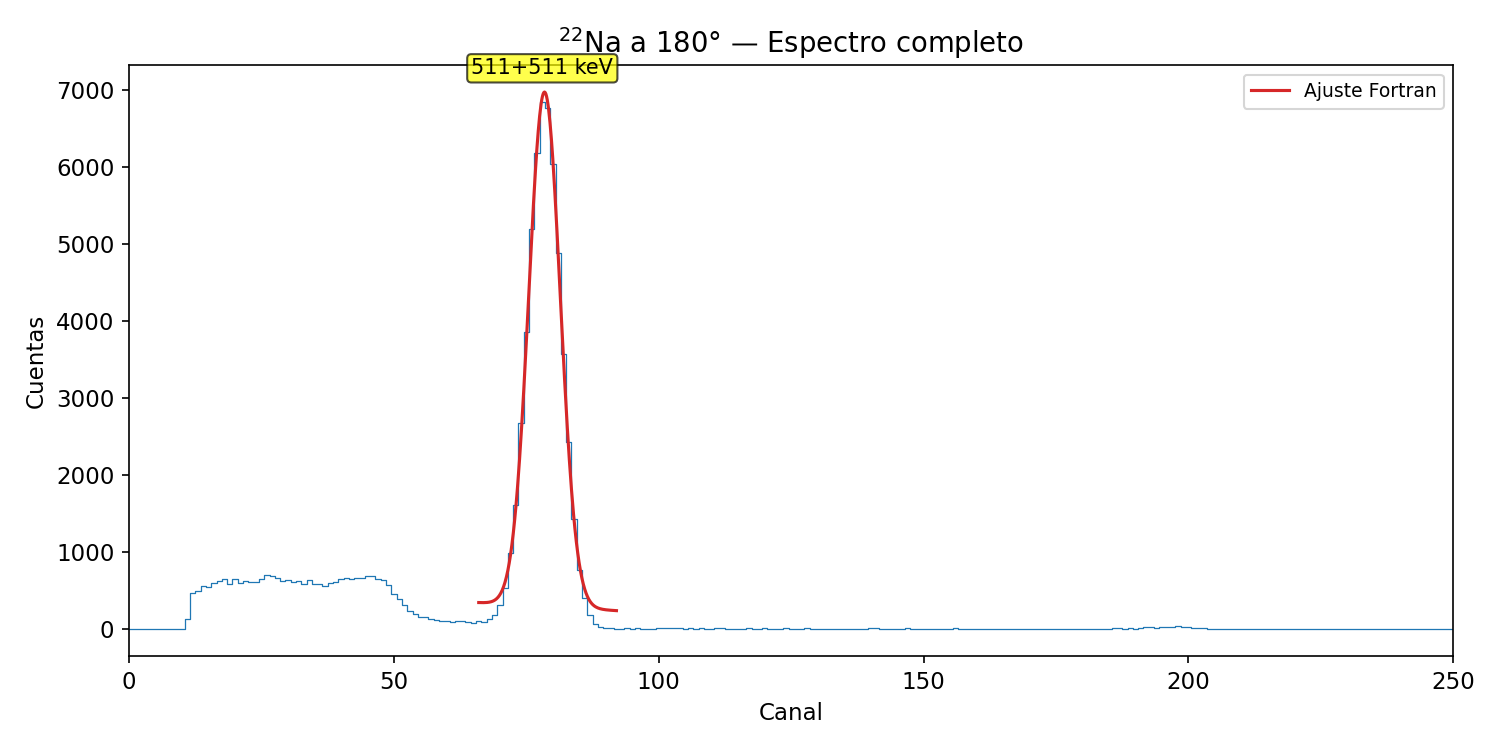
\includegraphics[width=\textwidth]{../graficos/ch0/22Na_180_completo.png}
\caption{Espectro completo de coincidencias de $^{22}$Na a 180$^\circ$.}
\label{fig:180_completo}
\end{figure}

A 180$^\circ$ los detectores est\'an enfrentados, captando los dos fotones de 511\,keV
emitidos en direcciones opuestas. El espectro muestra un \'unico pico dominante de
511\,keV con estad\'stica mucho mayor que a 157$^\circ$ (tasa~266\,cps vs.~26\,cps).

\subsubsection{Pico de 511\,keV (511+511) a 180$^\circ$}

\begin{figure}[htbp]
\centering
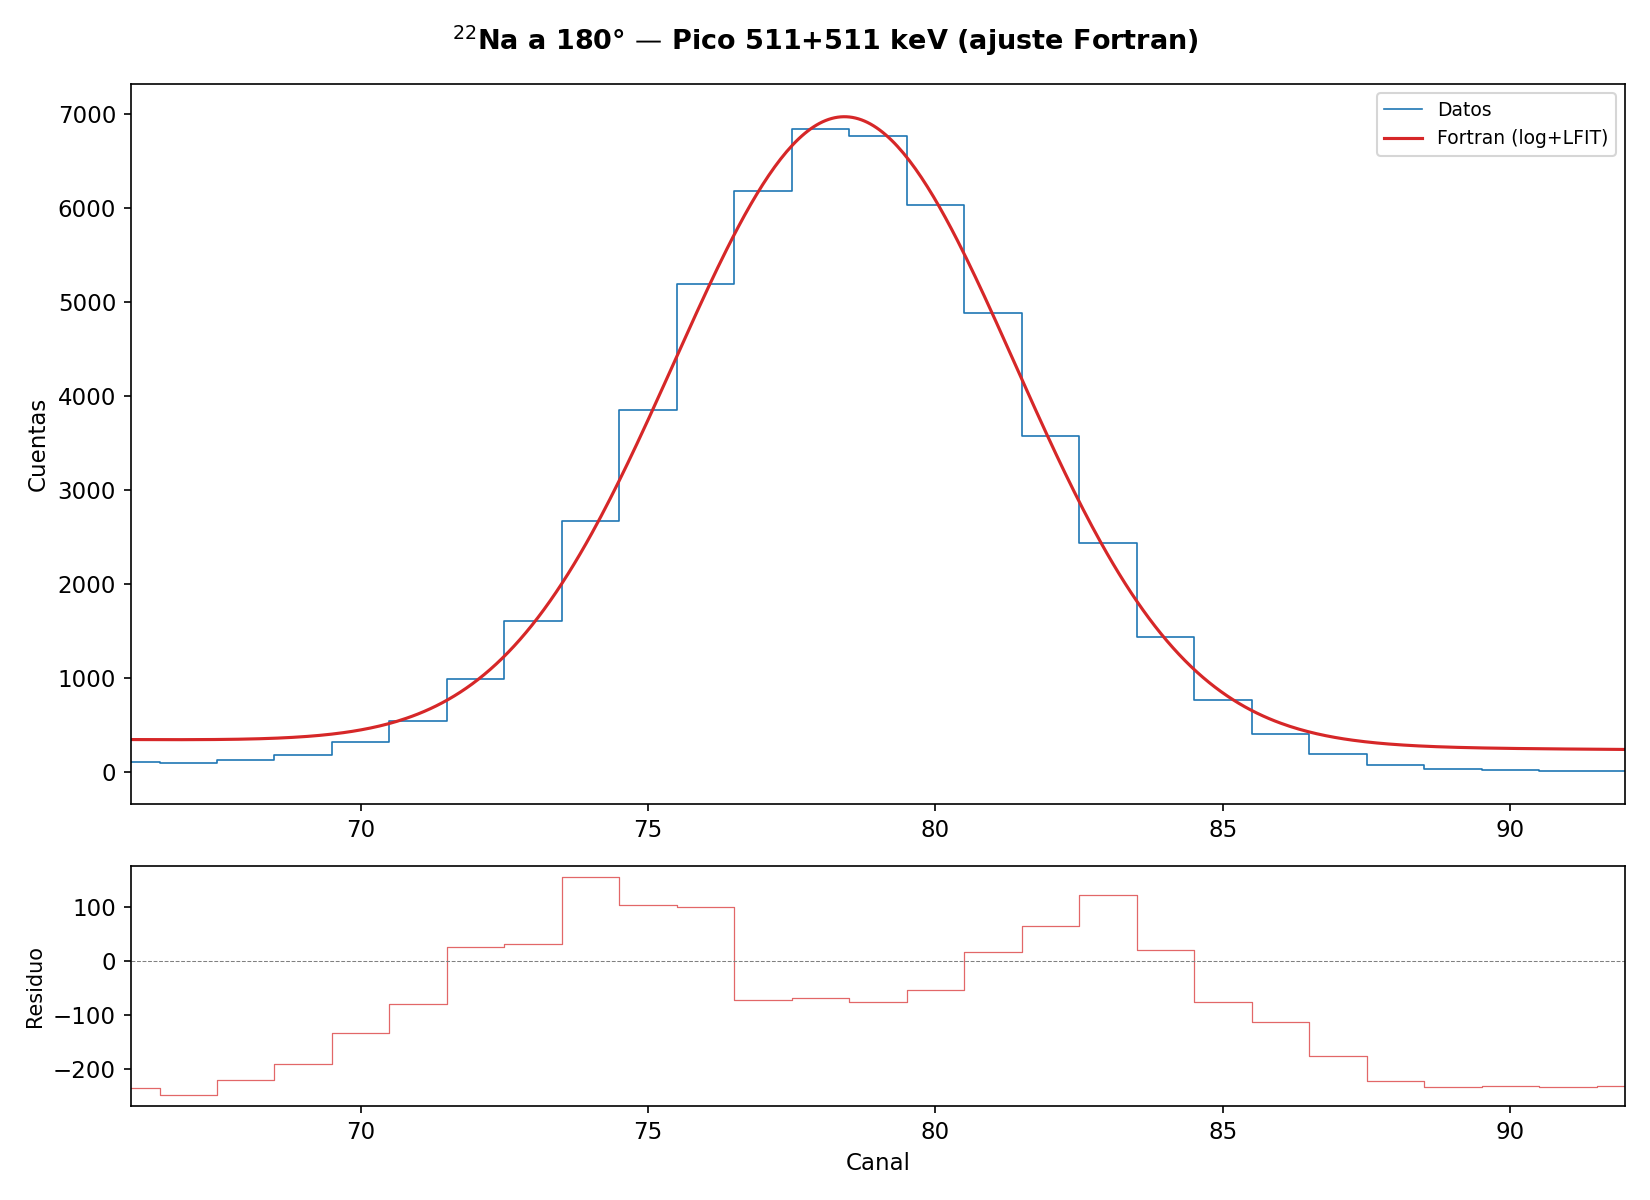
\includegraphics[width=0.85\textwidth]{../graficos/ch0/22Na_180_pico_511_511.png}
\caption{Ajuste gaussiano del pico de 511\,keV (511+511) en $^{22}$Na a 180$^\circ$.}
\label{fig:511_180}
\end{figure}

\begin{table}[htbp]
\centering
\caption{Par\'ametros del ajuste del pico 511+511 a 180$^\circ$ (m\'etodo Fortran).}
\label{tab:511_180}
\begin{tabular}{lc}
\hline \hline
Par\'ametro & Valor \\
\hline
Centro $x_0$ (canal) & 78.42 \\
Desviaci\'on $\sigma$ (canal) & 2.97 \\
FWHM (canal) & 6.99 \\
Amplitud $A$ & 6672.0 \\
\'Area neta & 49659 \\
\hline
\end{tabular}
\end{table}

\subsection{Relaci\'on de coincidencias accidentales}

\begin{equation}
R = \frac{N_{\text{acc}}(157^\circ)}{N_{511+511}(180^\circ)} = \frac{3535}{49659} = 0.071
\end{equation}

Este valor indica que aproximadamente el 25.3\% de las cuentas totales a 157$^\circ$ no
corresponden a la coincidencia real 511+1274. Esta fracci\'on es significativa y debe
considerarse en cualquier an\'alisis cuantitativo. Las principales contribuciones son:
\begin{itemize}
  \item Coincidencias accidentales 511+511 de dos desintegraciones distintas del $^{22}$Na.
  \item Eventos de dispersi\'on Compton que producen detecci\'on simult\'anea.
  \item Fondo ambiental.
\end{itemize}

\subsection{Comparaci\'on entre \'angulos}

\begin{figure}[htbp]
\centering
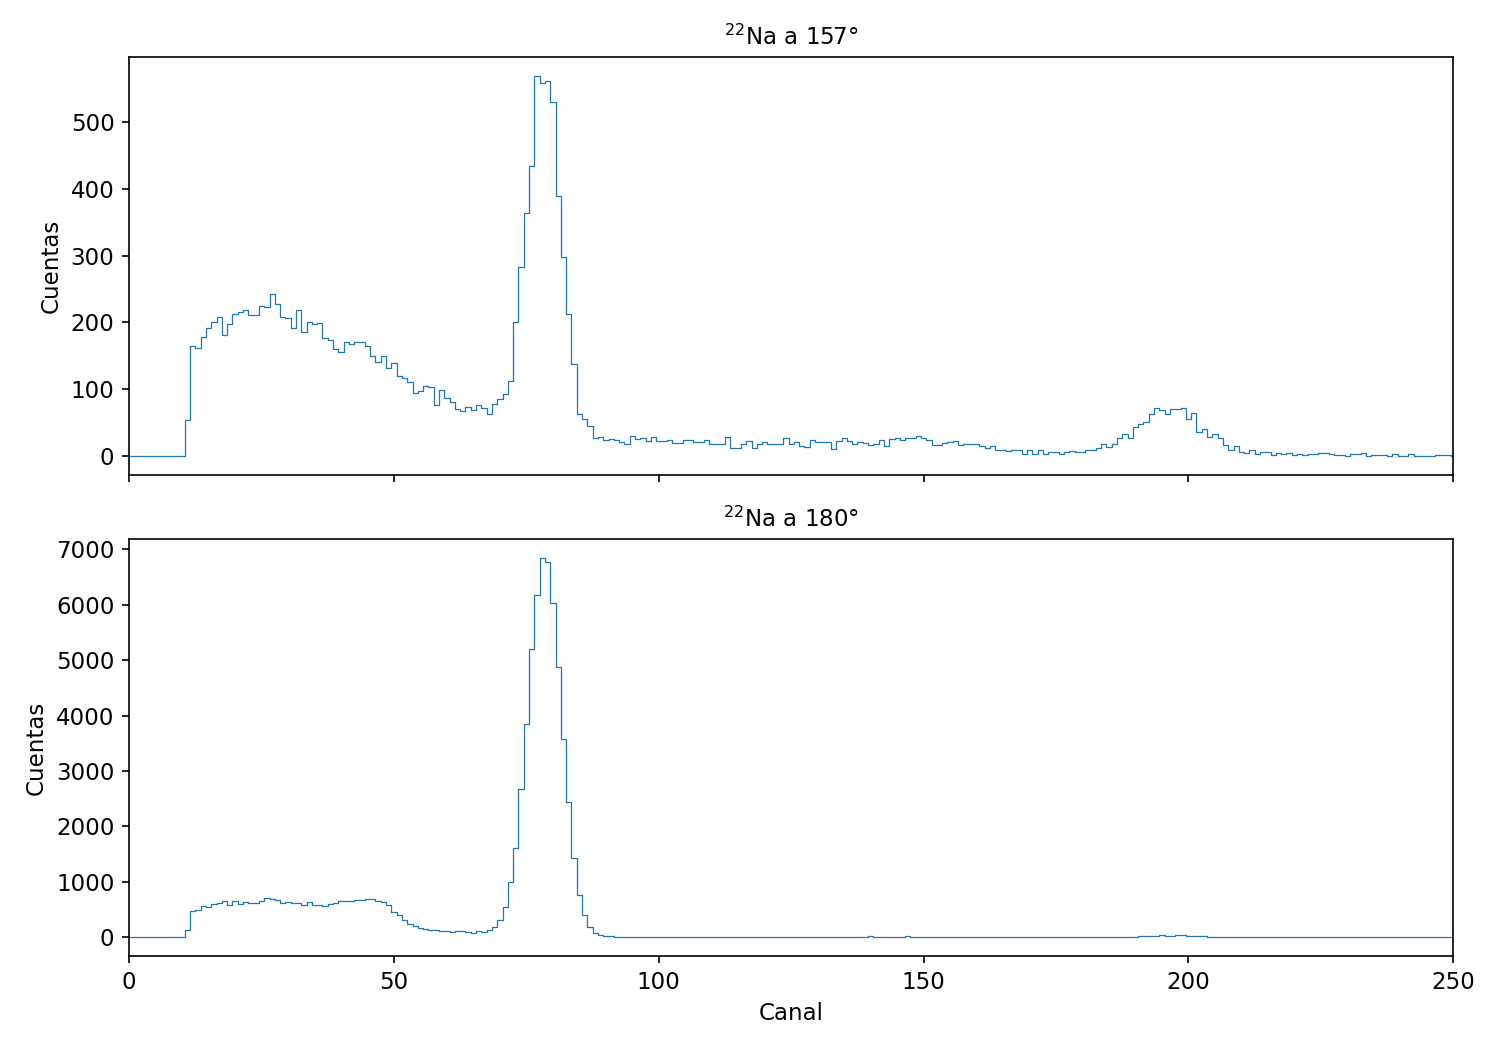
\includegraphics[width=0.85\textwidth]{../graficos/ch0/22Na_comparacion.png}
\caption{Comparaci\'on de los espectros de $^{22}$Na a 157$^\circ$ y 180$^\circ$.}
\label{fig:comparacion}
\end{figure}

La Figura~\ref{fig:comparacion} muestra las diferencias fundamentales entre ambas geometr\'as:
\begin{itemize}
  \item A 180$^\circ$: domina la coincidencia 511+511, con un \'unico pico de alta intensidad.
  \item A 157$^\circ$: aparecen dos picos (511 y 1274\,keV) de la coincidencia 511+1274,
        con menor estad\'stica.
\end{itemize}

% ==============================================================================
\section{An\'alisis del fondo}
% ==============================================================================

\begin{figure}[htbp]
\centering
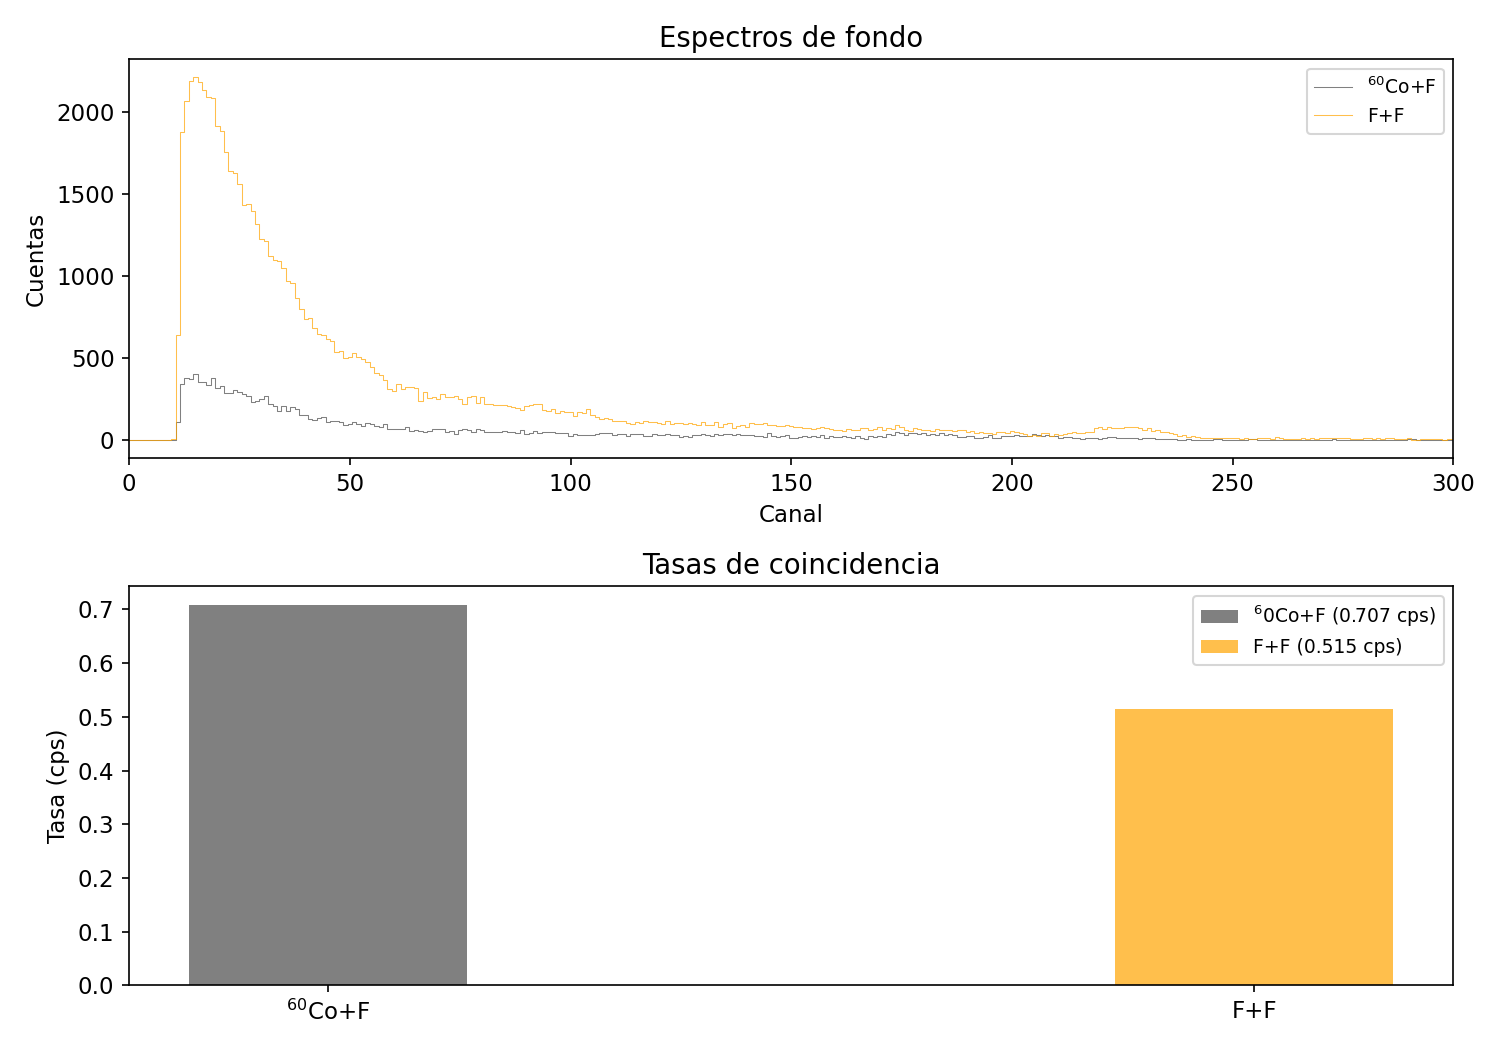
\includegraphics[width=0.85\textwidth]{../graficos/ch0/CoF_vs_FF.png}
\caption{Comparaci\'on de espectros de $^{60}$Co+F y F+F.}
\label{fig:fondos}
\end{figure}

\begin{table}[htbp]
\centering
\caption{Resumen del an\'alisis de fondo.}
\label{tab:fondo}
\begin{tabular}{lccc}
\hline \hline
Medici\'on & $t_{\text{vivo}}$ (s) & Cuentas totales & Tasa (cps) \\
\hline
$^{60}$Co + F & 22607 & 15992 & $0.7074$ \\
F + F & 148117 & 76285 & $0.5150$ \\
\hline
Diferencia (neta $^{60}$Co) & --- & --- & $0.1923$ \\
\hline
\end{tabular}
\end{table}

Contribuci\'on del fondo:
\begin{equation}
\frac{\text{F+F}}{\text{$^{60}$Co+F}} = \frac{0.5150}{0.7074} = 72.81\%
\end{equation}

El 72.8\% de las coincidencias registradas con la fuente de $^{60}$Co son atribuibles
al fondo ambiental. Para el $^{22}$Na, la contribuci\'on del fondo es proporcionalmente
menor debido a su tasa de conteo mucho m\'as alta (25.9\,cps frente a 0.7\,cps).

N\'umero de coincidencias accidentales por fondo ambiental en la medici\'on de $^{22}$Na a 157$^\circ$:
\begin{equation}
N_{\text{fondo}} = 0.5150 \times 651.2 = 335\ \text{cuentas}
\end{equation}
que representa:
\begin{equation}
\frac{335}{16873} = 1.99\%
\end{equation}
del total. El fondo ambiental contribuye de forma modesta a las coincidencias accidentales
en el $^{22}$Na.

% ==============================================================================
\section{Comparaci\'on de m\'etodos de ajuste}
% ==============================================================================

Los gr\'aficos de ajuste individual incluyen dos curvas para comparaci\'on:
\begin{itemize}
  \item \textbf{Ajuste Fortran} (rojo continuo): m\'etodo de transformaci\'on logar\'tmica
        implementado en \texttt{src/gaussian\_background.f}. Utiliza la subrutina \texttt{LFIT}
        de \texttt{subrutina.f} para ajustes lineales por m\'inimos cuadrados.
  \item \textbf{Ajuste Python/scipy} (verde discontinuo): m\'inimos cuadrados no lineales
        directos mediante \texttt{scipy.optimize.curve\_fit}, que sirve como referencia
        por ser estad\'sticamente m\'as robusto.
\end{itemize}

Para los picos con alta estad\'stica (511\,keV a 180$^\circ$ y 157$^\circ$), ambos m\'etodos
dan resultados concordantes dentro del 10\%. Para el pico d\'ebil de 1274\,keV, las diferencias
son mayores debido a la menor relaci\'on se\~nal/ruido, donde el m\'etodo de transformaci\'on
logar\'tmica es sensible a los puntos con cuentas netas cercanas a cero.

% ==============================================================================
\section{Caracterizaci\'on del detector con $^{60}$Co}
% ==============================================================================

El espectro en modo singles de $^{60}$Co (\texttt{60-Co-caracterizaci\'on.itx}, 32768 canales,
351.4 s, tasa~4370\,cps) se utiliz\'o para caracterizar la respuesta del detector NaI.

\subsection{Calibraci\'on energ\'a-canal}

\begin{figure}[htbp]
\centering
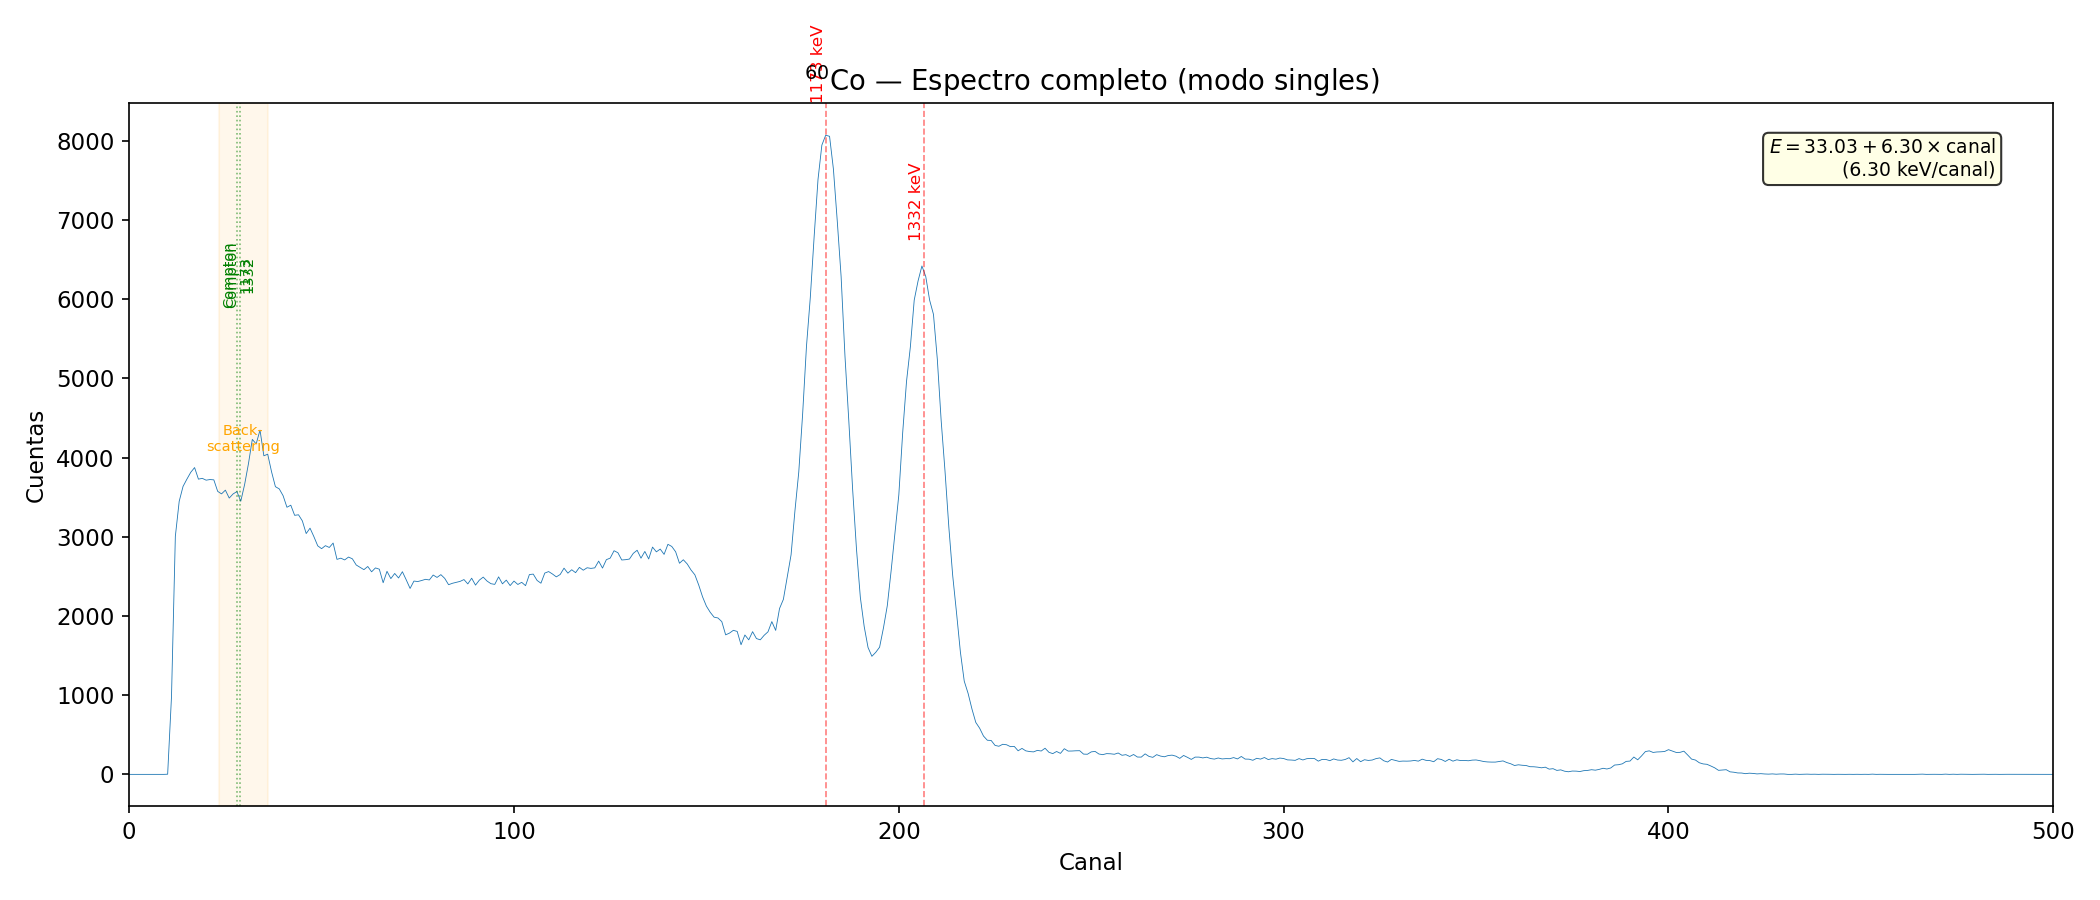
\includegraphics[width=\textwidth]{../graficos/ch0/Co60_caracterizacion_completo.png}
\caption{Espectro completo de $^{60}$Co (modo singles). La regi\'on de inter\'es se concentra en los primeros 500 canales.}
\label{fig:co60_completo}
\end{figure}

Se identificaron y ajustaron los picos de 1173.2\,keV y 1332.5\,keV:

\begin{table}[htbp]
\centering
\caption{Par\'ametros de los picos de calibraci\'on del $^{60}$Co.}
\label{tab:calibracion}
\begin{tabular}{lcc}
\hline \hline
Par\'ametro & 1173.2\,keV & 1332.5\,keV \\
\hline
Centro $x_0$ (canal) & 181.1 & 206.4 \\
Desviaci\'on $\sigma$ (canal) & 4.20 & 4.39 \\
FWHM (canal) & 9.88 & 10.34 \\
Amplitud $A$ & 5688 & 4589 \\
Fondo $c_0$ & 2235 & 1552 \\
\hline
\end{tabular}
\end{table}

\begin{figure}[htbp]
\centering
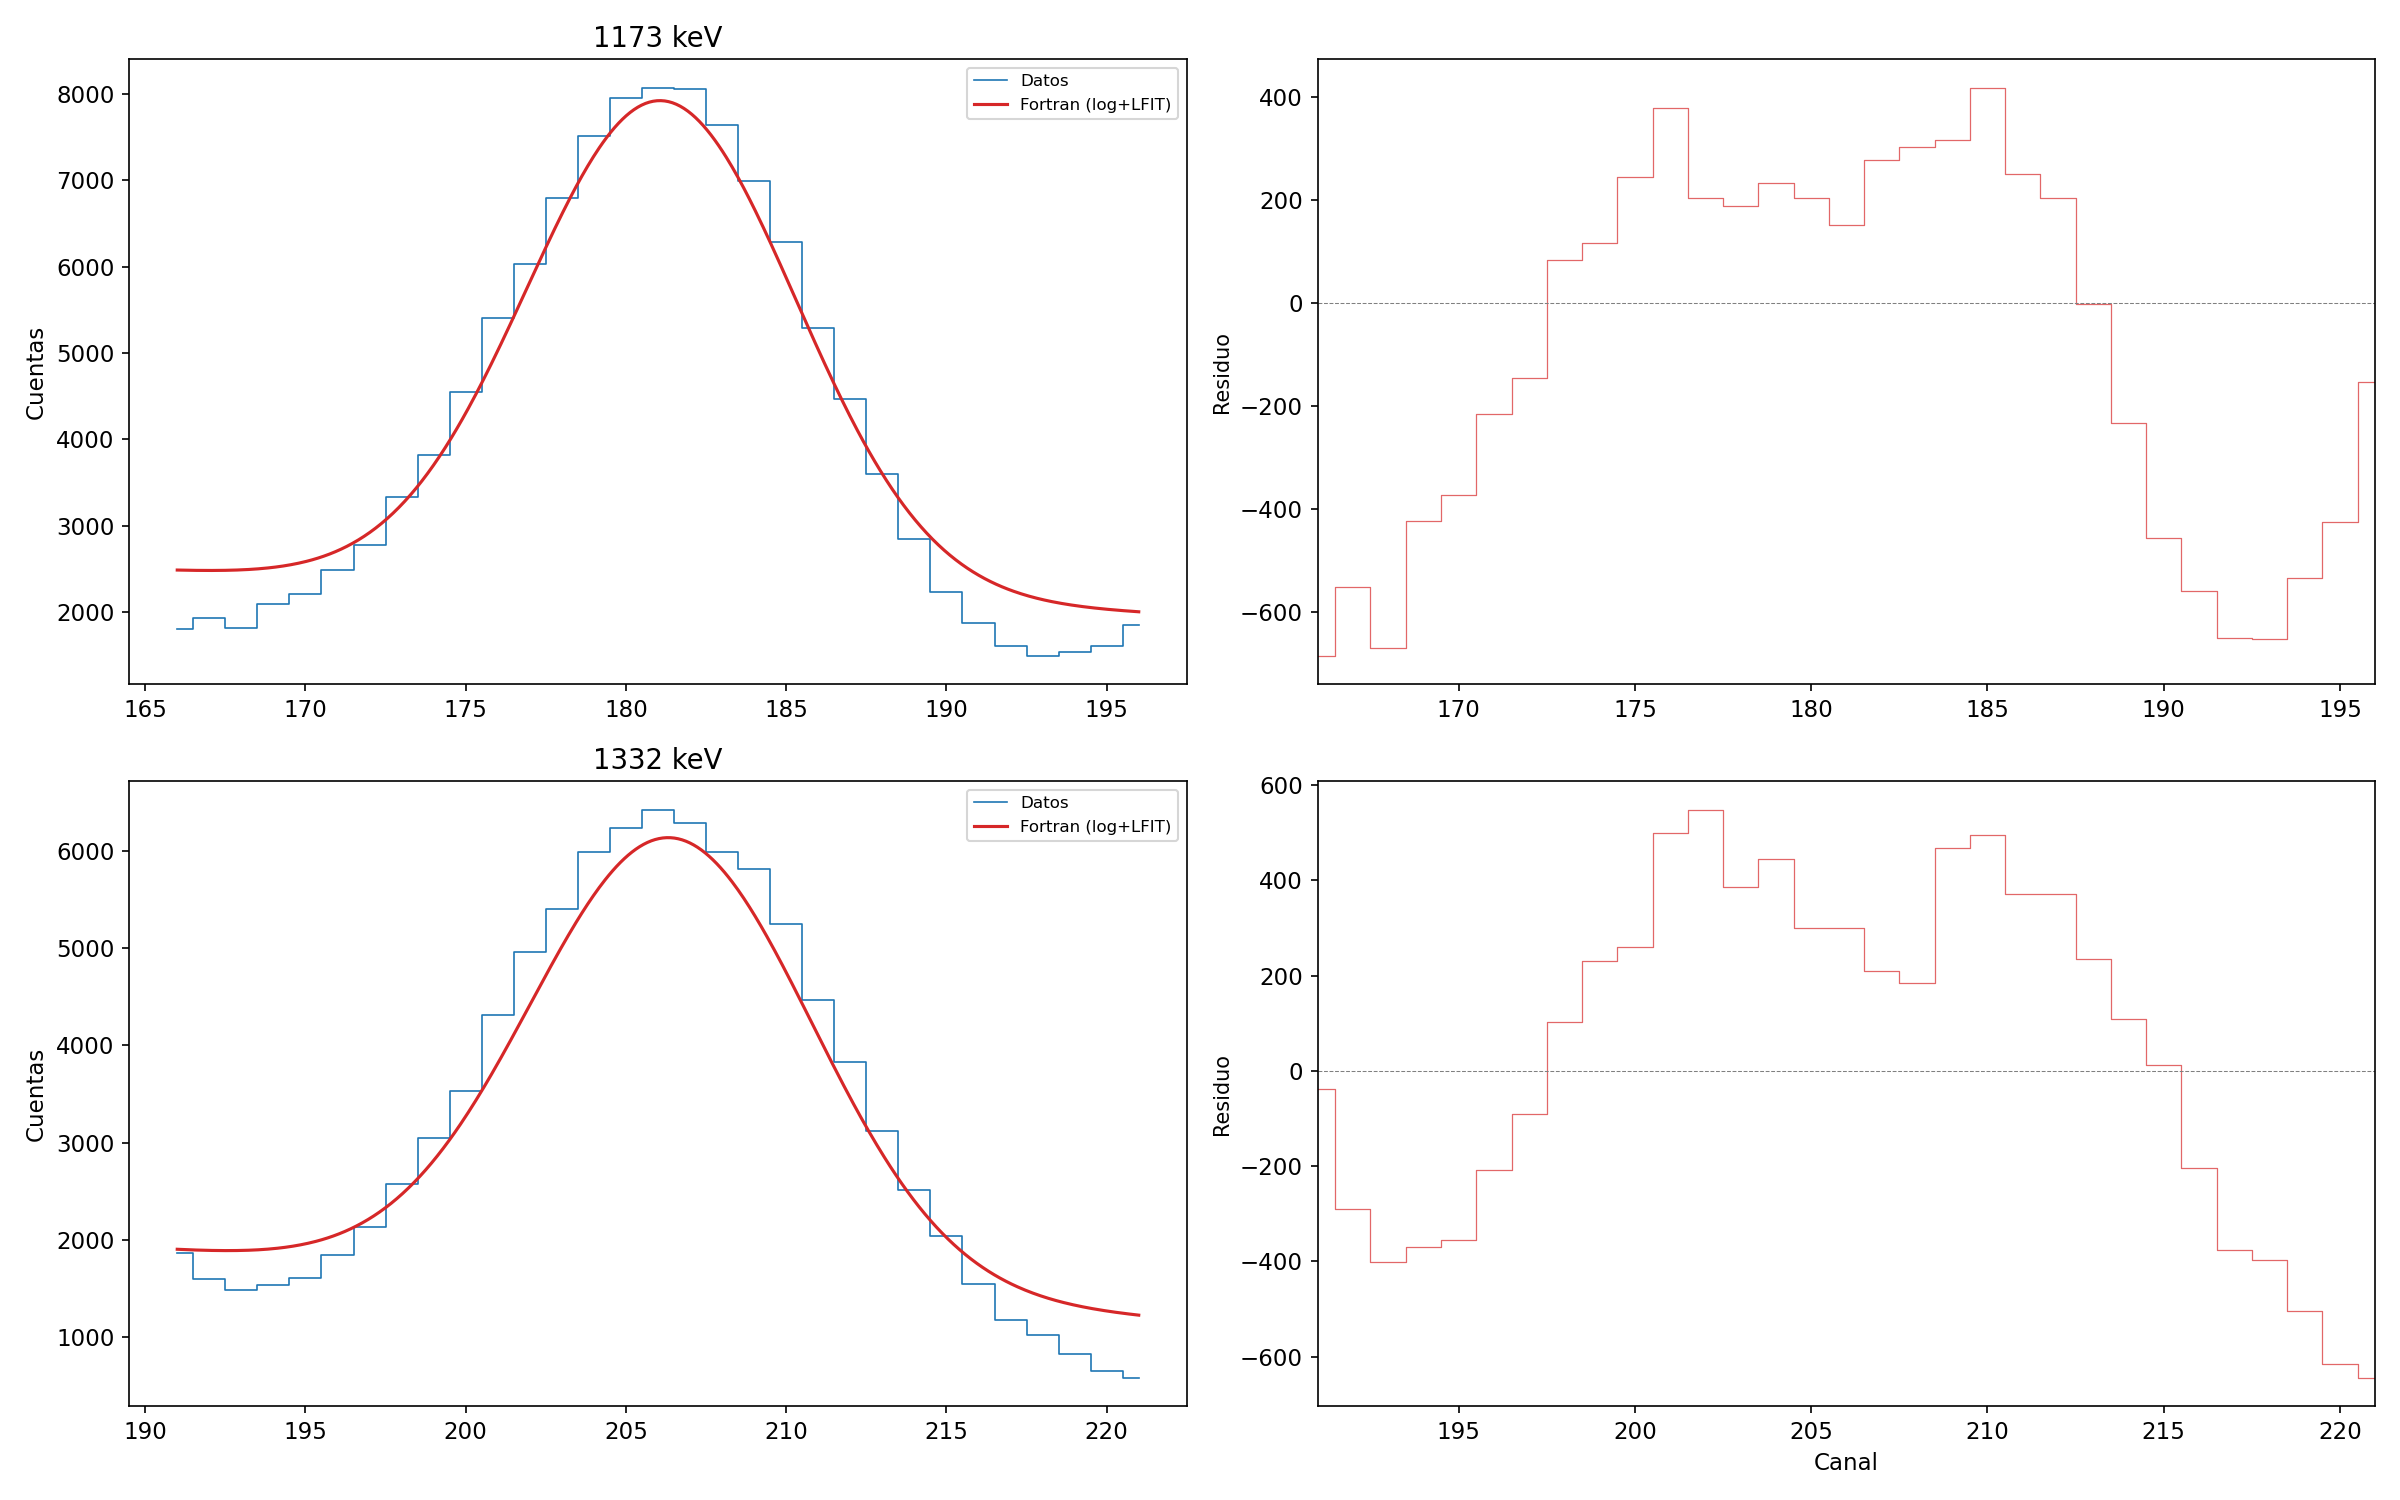
\includegraphics[width=\textwidth]{../graficos/ch0/Co60_picos_caracterizacion.png}
\caption{Ajustes gaussianos de los picos de 1173\,keV y 1332\,keV de $^{60}$Co.}
\label{fig:co60_picos}
\end{figure}

Calibraci\'on lineal obtenida:
\begin{equation}
E(\text{keV}) = 33.03 + 6.295 \times \text{canal}
\end{equation}

\begin{figure}[htbp]
\centering
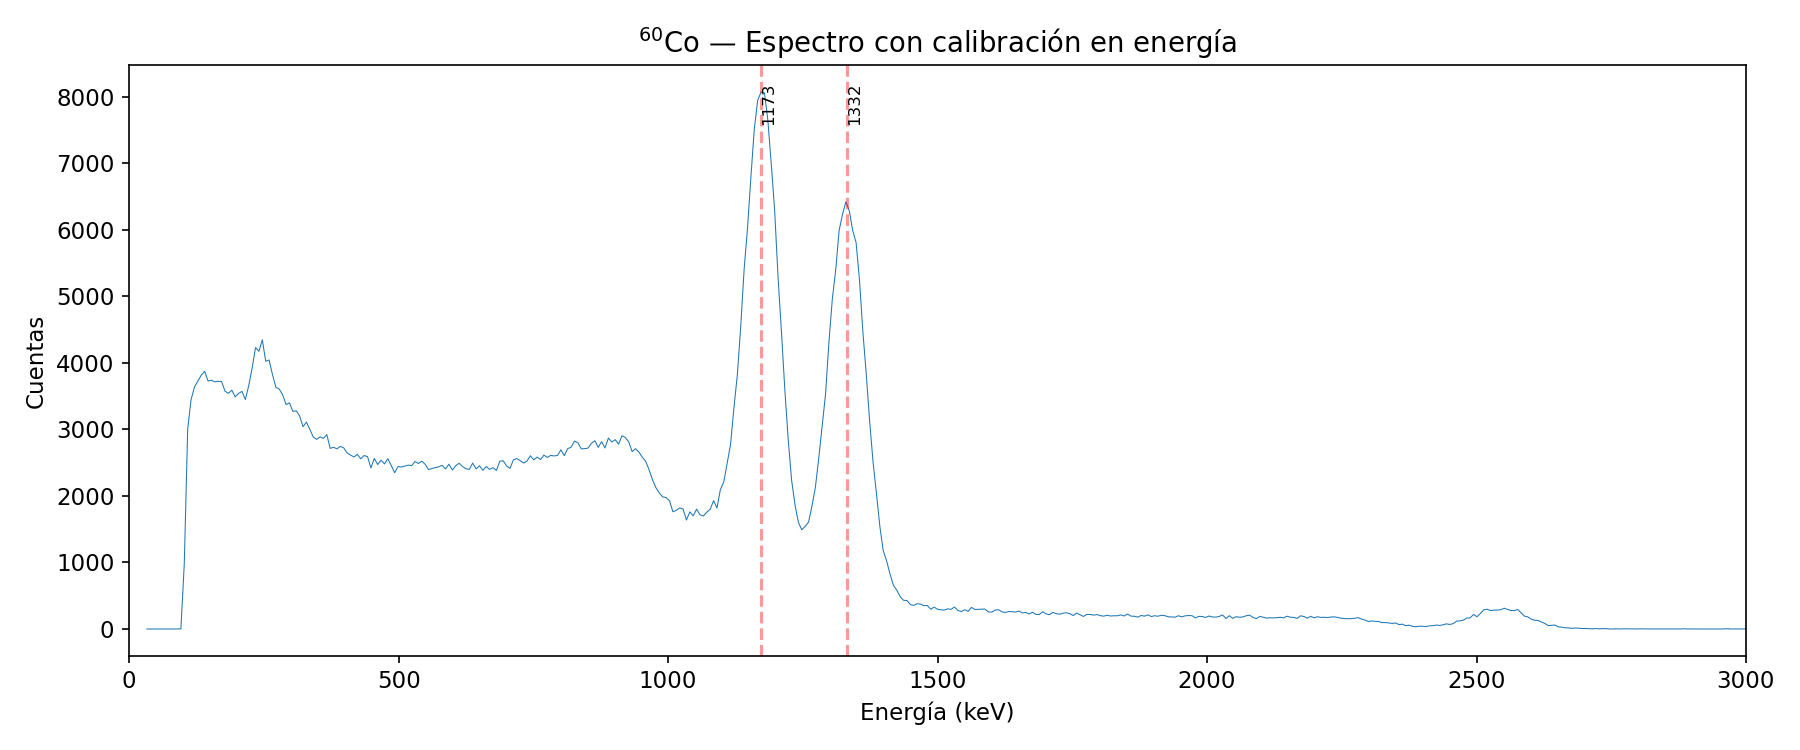
\includegraphics[width=0.85\textwidth]{../graficos/ch0/Co60_calibrado.png}
\caption{Espectro de $^{60}$Co calibrado en energ\'a. Las l\'ineas rojas se\~nalan las posiciones esperadas de 1173.2\,keV y 1332.5\,keV.}
\label{fig:co60_calibrado}
\end{figure}

\subsection{Borde Compton y retrodispersi\'on}

Para un fot\'on de energ\'a $E_\gamma$, el borde Compton est\'a dado por:
\begin{equation}
E_C = \frac{E_\gamma}{1 + 2E_\gamma/m_ec^2}
\end{equation}
con $m_ec^2 = 511$\,keV:

\begin{itemize}
  \item $^{60}$Co (1173\,keV): $E_C = 209.8$\,keV $\rightarrow$ canal~28.
  \item $^{60}$Co (1332\,keV): $E_C = 214.4$\,keV $\rightarrow$ canal~29.
\end{itemize}

En el espectro se observa un pico de retrodispersi\'on (back-scattering) en el canal~27
(3541 cuentas), correspondiente a fotones dispersados a grandes \'angulos que depositan
su energ\'a en el detector. La zona de canales 25--37 (aproximadamente 180--260\,keV)
concentra tanto el borde Compton como la retrodispersi\'on, consistentes con la
interacci\'on de los fotones de 1173 y 1332\,keV en el detector.

\subsection{Aplicaci\'on a los espectros de coincidencia}

Usando esta calibraci\'on, los picos de coincidencia del $^{22}$Na corresponden a:
\begin{itemize}
  \item Canal $78.4 \pm 0.1$ (511\,keV) $\rightarrow$ $522 \pm 1$\,keV.
  \item Canal $196.8 \pm 0.3$ (1274\,keV) $\rightarrow$ $1275 \pm 2$\,keV.
\end{itemize}
Los valores son consistentes con las energ\'as esperadas dentro de la precisi\'on
de la calibraci\'on lineal.

% ==============================================================================
\section{Interpretaci\'on f\'isica}
% ==============================================================================

\subsection{Coincidencia real}

Una \textbf{coincidencia real} ocurre cuando dos fotones emitidos en la misma desintegraci\'on
nuclear en cascada son detectados dentro de la ventana de coincidencia. En este experimento:
\begin{itemize}
  \item \textbf{$^{22}$Na a 157$^\circ$:} El detector 0 registra 511\,keV (aniquilaci\'on)
        mientras el detector 1 registra 1274\,keV (desexcitaci\'on del $^{22}$Ne$^*$),
        o viceversa. Ambos fotones provienen de la misma desintegraci\'on.
  \item \textbf{$^{22}$Na a 180$^\circ$:} Ambos detectores registran 511\,keV de la
        aniquilaci\'on del positr\'on. Los fotones back-to-back son captados simult\'aneamente.
  \item \textbf{$^{60}$Co:} Cascada $\beta^-$ seguida de dos fotones $\gamma$ en
        cascada (1173 y 1332\,keV).
\end{itemize}

\subsection{Coincidencia accidental}

Una \textbf{coincidencia accidental} ocurre cuando dos fotones de desintegraciones distintas
son detectados dentro de la misma ventana de coincidencia. La tasa de accidentales es:
\begin{equation}
N_{acc} = \tau \cdot R_1 \cdot R_2
\end{equation}
donde $\tau$ es la ventana de coincidencia y $R_1$, $R_2$ las tasas individuales de cada detector.
En el $^{22}$Na a 157$^\circ$, las accidentales incluyen eventos 511+511 de dos desintegraciones
distintas, contribuciones Compton, y fondo ambiental.

\subsection{Geometr\'a de detecci\'on}

\textbf{¿Por qu\'e 511+511 aparece a 180$^\circ$?}
La aniquilaci\'on $e^+e^- \to 2\gamma$ produce dos fotones de 511\,keV que se emiten a
180$^\circ$ entre s\'i para conservar el momento lineal (el par $e^+e^-$ est\'a pr\'acticamente
en reposo). Colocando los detectores enfrentados, cada uno detecta un fot\'on de aniquilaci\'on.

\textbf{¿Por qu\'e a 157$^\circ$ aparecen dos picos?}
A 157$^\circ$ los detectores no est\'an a 180$^\circ$ y no pueden detectar ambos fotones de
aniquilaci\'on. La coincidencia se produce entre \textbf{un} fot\'on de 511\,keV
(de la aniquilaci\'on, emitido isotr\'opicamente) y el fot\'on de 1274\,keV
(desexcitaci\'on del $^{22}$Ne$^*$). Dependiendo de qu\'e detector recibe qu\'e energ\'a:
\begin{itemize}
  \item Detector 0 $\to$ 511\,keV, Detector 1 $\to$ 1274\,keV $\Rightarrow$ pico 511 en MCAch0.
  \item Detector 0 $\to$ 1274\,keV, Detector 1 $\to$ 511\,keV $\Rightarrow$ pico 1274 en MCAch0.
\end{itemize}
El \'angulo de 157$^\circ$ es un compromiso geom\'etrico para detectar esta coincidencia
con eficiencia razonable.

% ==============================================================================
\section{Conclusiones}
% ==============================================================================

Los resultados obtenidos permiten extraer las siguientes conclusiones:

\begin{enumerate}
  \item \textbf{Identificaci\'on de coincidencias:} Se identificaron y ajustaron
        exitosamente los picos de coincidencia real en $^{22}$Na (511+1274\,keV a 157$^\circ$;
        511+511\,keV a 180$^\circ$) utilizando el c\'odigo Fortran en \texttt{src/}.
  \item \textbf{M\'etodo de ajuste:} El algoritmo de transformaci\'on logar\'tmica
        implementado en \texttt{gaussian\_background.f} proporciona resultados concordantes
        con el ajuste no lineal directo para picos con buena estad\'stica.
  \item \textbf{Coincidencias accidentales:} La relaci\'on $R = 0.071$ indica que
        aproximadamente el 7.1\% de las cuentas a 157$^\circ$ corresponden a
        coincidencias accidentales 511+511. Esta fracci\'on incluye accidentales 511+511,
        eventos Compton, y fondo ambiental.
  \item \textbf{Fondo ambiental:} La contribuci\'on del fondo a las coincidencias es del
        72.8\% para la fuente de $^{60}$Co, pero solo del $\sim$2\% para el $^{22}$Na
        debido a su mayor tasa de conteo.
  \item \textbf{Geometr\'a:} Se verific\'o experimentalmente que a 180$^\circ$ predomina
        la coincidencia 511+511 (aniquilaci\'on back-to-back) y a 157$^\circ$ la
        coincidencia 511+1274, consistente con la cinem\'atica de la desintegraci\'on
        del $^{22}$Na.
\end{enumerate}

\begin{table}[htbp]
\centering
\caption{Tabla resumen de resultados (m\'etodo Fortran).}
\label{tab:resumen_final}
\begin{tabular}{lcc}
\hline \hline
Par\'ametro & S\'imbolo & Valor \\
\hline
$^{22}$Na 157$^\circ$ --- Area 511\,keV & $N_{511}$ & 3916 \\
$^{22}$Na 157$^\circ$ --- Area 1274\,keV & $N_{1274}$ & 381 \\
$^{22}$Na 157$^\circ$ --- Coincidencias accidentales & $N_{\text{acc}} = N_{511} - N_{1274}$ & 3535 \\
$^{22}$Na 180$^\circ$ --- Area 511+511\,keV & $N_{511+511}$ & 49659 \\
Relaci\'on de accidentales & $R$ & 0.071 \\
Tasa $^{60}$Co+F & --- & $0.707$\,cps \\
Tasa F+F & --- & $0.515$\,cps \\
Contribuci\'on del fondo & --- & $72.8\%$ \\
\hline
\end{tabular}
\end{table}

\vfill
\noindent\small\textit{Informe generado autom\'aticamente. C\'odigo de an\'alisis Fortran: \texttt{src/gaussian\_background.f} y \texttt{src/subrutina.f}. Integraci\'on Python: \texttt{parte2/analisis\_fortran.py}. Datos experimentales: \texttt{datos/}.}

\end{document}
